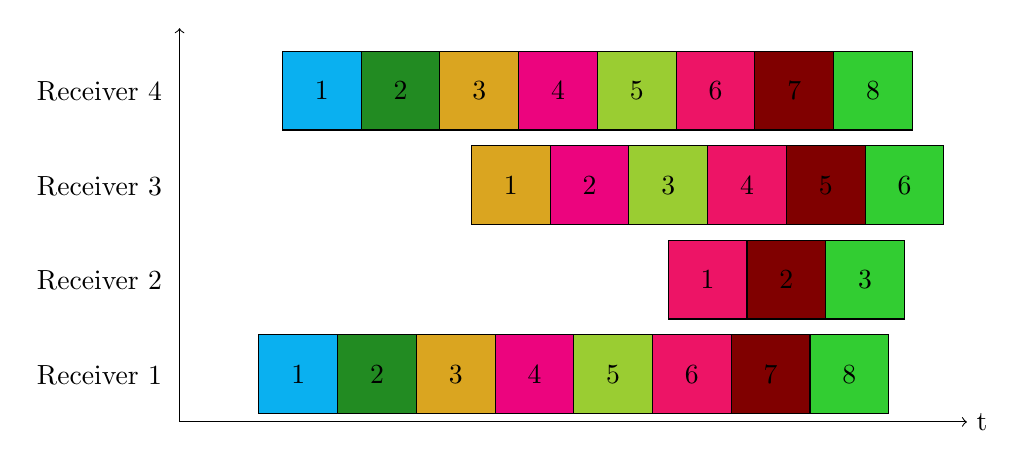
\begin{tikzpicture}[x=1cm, y=1cm]
  \tikzset{
    sample/.style={minimum width=10mm, minimum height=10mm, anchor=south west, draw=black},
    label/.style={anchor=east},
  }

  % time axis
  \draw[->]
  (0, 0) --
  (10, 0) node[anchor=west]{t};

  % other axis
  \draw[->]
  (0, 0) --
  (0, 5);

  % Receiver 1
  \draw
  (1.0, 0.1) node[sample, fill=ProcessBlue]{1}
  +(1, 0) node[sample, fill=ForestGreen]{2}
  +(2, 0) node[sample, fill=Goldenrod]{3}
  +(3, 0) node[sample, fill=RubineRed]{4}
  +(4, 0) node[sample, fill=YellowGreen]{5}
  +(5, 0) node[sample, fill=WildStrawberry]{6}
  +(6, 0) node[sample, fill=Maroon]{7}
  +(7, 0) node[sample, fill=LimeGreen]{8};

  % Receiver 2
  \draw
  (6.2, 1.3) node[sample, fill=WildStrawberry]{1}
  +(1, 0) node[sample, fill=Maroon]{2}
  +(2, 0) node[sample, fill=LimeGreen]{3};

  % Receiver 3
  \draw
  (3.7, 2.5) node[sample, fill=Goldenrod]{1}
  +(1, 0) node[sample, fill=RubineRed]{2}
  +(2, 0) node[sample, fill=YellowGreen]{3}
  +(3, 0) node[sample, fill=WildStrawberry]{4}
  +(4, 0) node[sample, fill=Maroon]{5}
  +(5, 0) node[sample, fill=LimeGreen]{6};

  % Receiver 4
  \draw
  (1.3, 3.7) node[sample, fill=ProcessBlue]{1}
  +(1, 0) node[sample, fill=ForestGreen]{2}
  +(2, 0) node[sample, fill=Goldenrod]{3}
  +(3, 0) node[sample, fill=RubineRed]{4}
  +(4, 0) node[sample, fill=YellowGreen]{5}
  +(5, 0) node[sample, fill=WildStrawberry]{6}
  +(6, 0) node[sample, fill=Maroon]{7}
  +(7, 0) node[sample, fill=LimeGreen]{8};

  \draw
  (-0.1, 0.6) node[label]{Receiver 1}
  (-0.1, 1.8) node[label]{Receiver 2}
  (-0.1, 3.0) node[label]{Receiver 3}
  (-0.1, 4.2) node[label]{Receiver 4};
\end{tikzpicture}
